\section{Integral im $\R^n$}
\begin{satz}[Fubini] Sei $Q = [a, b]$ x $[c, d] \subset \R^2$ und sei $f \in C^0$.\\
Dann kann das Integral von $f$ über $Q$, iterativ durch 1-dimensionale  Integration bestimmt werden:
\[
	\int_Q f \, d\mu = 
	\int_a^b \left( \int_c^d f(x, y) \, dy \right) \, dx = 
	\int_c^d \left( \int_a^b f(x, y) \, dx \right) \, dy
\]
\end{satz}

% Übung aus Analysis 2 - Serie 10
\textbf{Bsp. Bestimme die Integrationsgrenzen von $\Omega$ für $f(x, y)$}\\
1) 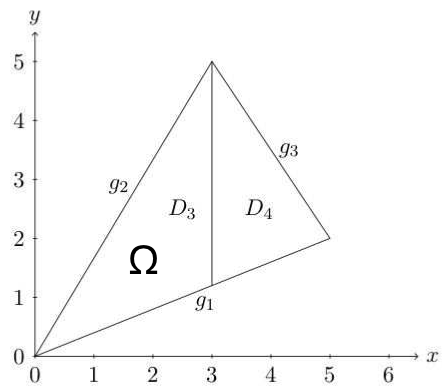
\includegraphics[scale=1.0]{doppelintegral_1.png} \hspace{1cm} 2) 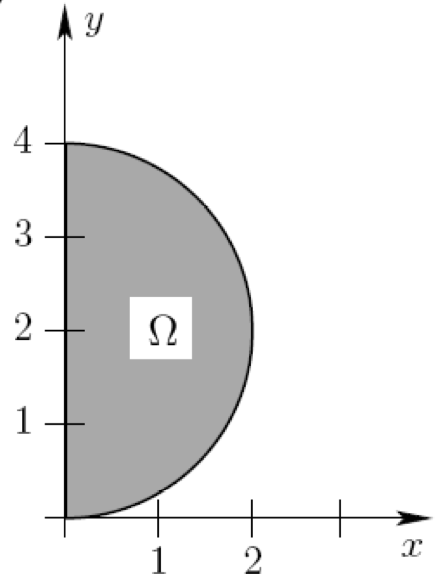
\includegraphics[scale=0.7]{doppelintegral_2.png}
\begin{enumerate}[leftmargin=0.5cm]
	\item \textbf{Integration des Dreiecks zuerst nach y dann nach x}
	\begin{enumerate}[leftmargin=0.3cm]
		\item Zuerst Geradengleichungen aufstellen:\\
		$g_1: y = \frac{2}{5}x$, $g_2: y = \frac{5}{3}x$, $g_3: y = \frac{19}{2} - \frac{3}{2}x$

		\item Bei der Integration zuerst nach y, müssen wir für jedes $x$, den entsprechenden Bereich für $y$ in der Form:\\
		$\phi_1(x) \leq y \leq \phi_2(y)$ angeben.
		Dazu wird $\Omega$ in $D_3$ und $D_4$ unterteilt und benutzen die Geradengleichungen:\\
		$D_3 = \{ (x, y): 0 \leq x \leq 3, \frac{2}{5}x \leq y \leq \frac{5}{3}x \}$\\
		$D_4 = \{ (x, y): 3 \leq x \leq 5, \frac{2}{5}x \leq y \leq \frac{19}{2} - \frac{3}{2}x \}$

		\item Einsetzen in Integral:
		\[\hspace{-0.8cm}\int_{\Omega} f(x, y) \, d\mu = 
		\int_0^3 \int_{\frac{2}{5}x}^{\frac{5}{3}x} f(x, y) \, dy \, dx +
		\int_3^5 \int_{\frac{2}{5}x}^{\frac{19}{2} - \frac{3}{2}x} f(x, y) \, dy \, dx\]
	\end{enumerate}

	\item \textbf{Integration des Halbkreis zuerst nach x dann nach y}
	\begin{enumerate}[leftmargin=0.3cm]
		\item Kreisgleichung hinschreiben: $x^2 + (y -2)^2 = 4$

		\item Bei der Integration zuerst nach x, müssen wir für jedes $y$, den entsprechenden Bereich für $x$ in der Form:\\
		$\phi_1(y) \leq x \leq \phi_2(y)$ angeben. Es gilt: $x = \sqrt{4 - (y-2)^2}$

		\item Einsetzen in Integral:
		\[\int_{\Omega} f(x, y) \, d\mu = \int_0^5 \int_0^{\sqrt{4 - (y-2)^2}} f(x, y) \, dx \, dy\]
	\end{enumerate}
\end{enumerate}

